\documentclass{beamer}
\usetheme{Madrid}
\usecolortheme{beaver}
\usefonttheme{serif}
\setbeamertemplate{footline}[page number]{}
\setbeamertemplate{navigation symbols}{}

\definecolor{burgundy}{rgb}{0.82, 0.1, 0.26}

\begin{document}
	
\title
{
	\texttt{bencherl}: A scalability benchmark suite for Erlang/OTP
}

\author
{
	Stavros Aronis\inst{1} \and
	Nikolaos Papaspyrou\inst{2} \and
	\textcolor{burgundy}{Katerina Roukounaki}\inst{2} \and
	Konstantinos Sagonas\inst{1,2} \and
	Yiannis Tsiouris\inst{2} \and
	Ioannis Venetis\inst{2}
}

\institute
{
	\inst{1}%
	Department of Information Technology, Uppsala University, Sweden
	\and
	\inst{2}%
	School of Electrical and Computer Engineering, National Technical University of Athens, Greece
}

\date
{Erlang Workshop 2012, Copenhagen}

\begin{frame}
	\titlepage
\end{frame}

\begin{frame}{What are benchmarks and benchmark suites?}
	\begin{itemize}[]
		\item {\bf Benchmarks} are programs that attempt to assess the performance of a piece of software or hardware.
		\item {\bf Benchmark suites} are are tools that can be used to run benchmarks in an automatic way, and then collect and analyze the measurements.
		\item Benchmark suites usually come with an initial collection of benchmarks that can be enhanced.  
	\end{itemize}

\end{frame}

\begin{frame}{What benchmark suites are out there?}
	\begin{itemize}[]
		\item {\bf Haskell}: nofib, nobench, fibon, Criterion, HaBench
		\item {\bf Java}: DaCapo benchmark suite
		\item {\bf Erlang}: Basho Bench
	\end{itemize}
\end{frame}

\begin{frame}{What is \texttt{bencherl}?}
	\begin{block}{}
	\texttt{bencherl} is a publicly available scalability benchmark suite for Erlang applications, as well as for the Erlang/OTP distribution itself.
	\end{block}
\end{frame}

\begin{frame}{What was the motivation behind \texttt{bencherl}?}
	\begin{block}{}
	"I thought my Erlang program was 100\% parallelizable, but when I made it parallel and ran it on a machine with N cores, the speedup I got was much lower compared to N."
	\end{block}
	\begin{center}
	    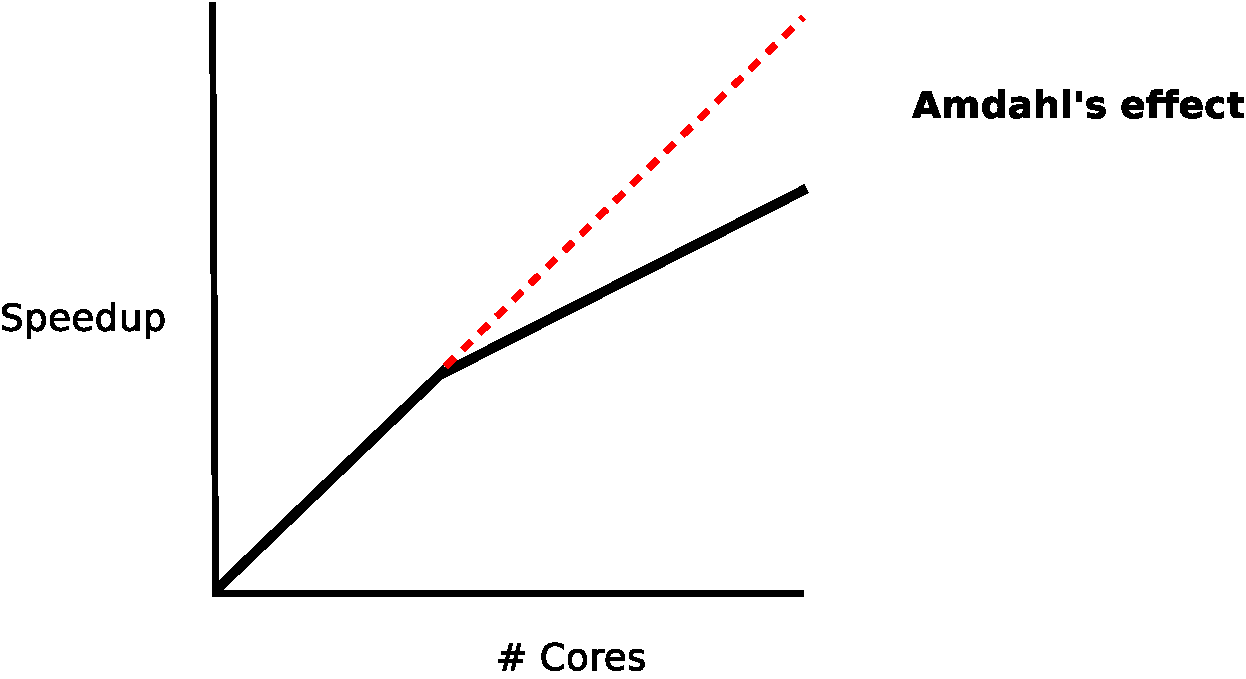
\includegraphics[width=0.5\linewidth]{figures/amdahls.pdf}
	\end{center}
	Not being able to take advantage of all available cores matters, especially on big multicores.
\end{frame}

\begin{frame}{What are the dimensions of the runtime environment that affect scalability?}
	\begin{itemize}
		\item {\bf Number of nodes}
		\begin{itemize}\item The number of Erlang nodes that run the application\end{itemize}
		\item {\bf Number of cores}
        \begin{itemize}\item The number of CPU cores used by each Erlang node\end{itemize}
 		\item {\bf Number of schedulers}
        \begin{itemize}\item The number of OS scheduler processes that each Erlang node starts\end{itemize}
 		\item {\bf Erlang/OTP release and flavor}
        \begin{itemize}\item The \texttt{erl} program that is used to start each Erlang node\end{itemize}
 		\item {\bf \texttt{erl} command-line arguments}
        \begin{itemize}\item The options that are passed to the \texttt{erl} program that is used to start eacj Erlang node\end{itemize}
 	\end{itemize}
	\begin{block}{Runtime environment}
		A point in the multi-dimensional space defined by the afore-mentioned dimensions.
	\end{block}
\end{frame}

\begin{frame}{What does \texttt{bencherl} look like?}
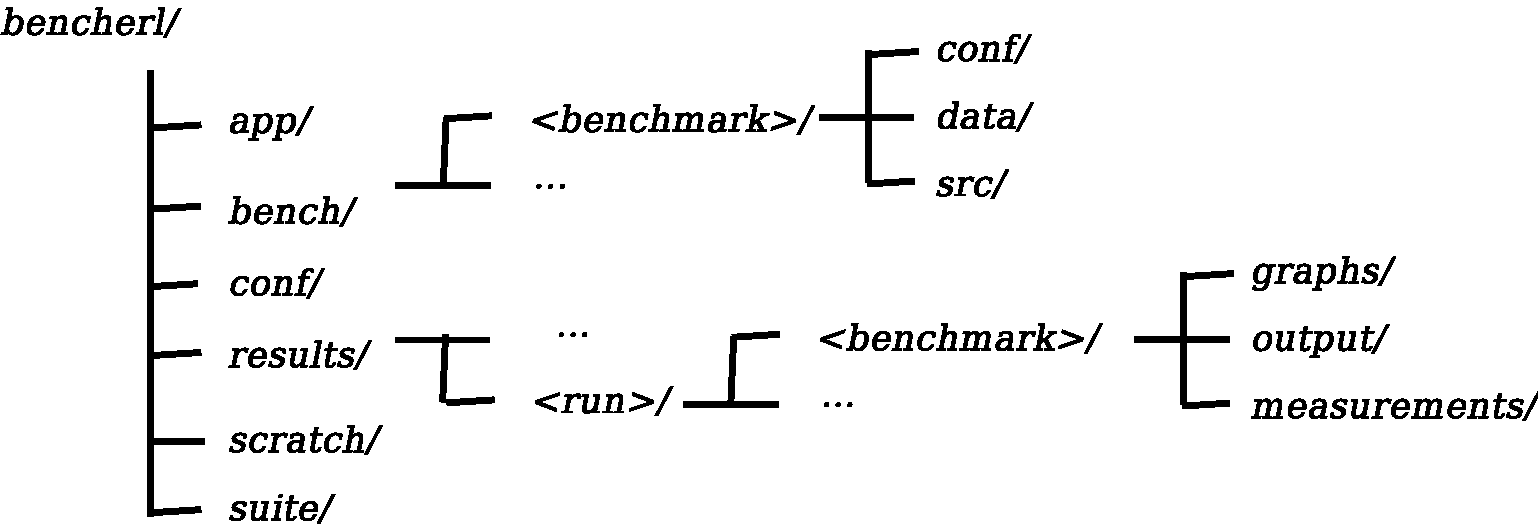
\includegraphics[width=\linewidth]{figures/structure.pdf}
	\begin{itemize}
		\item \texttt{app}: benchmarked applications
		\item \texttt{bench}: benchmarks
		\item \texttt{conf}: \texttt{bencherl} global configuration files
		\item \texttt{results}: results of \texttt{bencherl} runs 
			\begin{itemize}
				\item \texttt{graphs}: scalability graphs
				\item \texttt{measurements}: scalability measurements
				\item \texttt{output}: benchmark output
			\end{itemize}
		\item \texttt{scratch}: temporary files
		\item \texttt{suite}: benchmarking infrastructure
	\end{itemize}
\end{frame}

\begin{frame}{What is the architecture of \texttt{bencherl}?}
	\begin{center}
		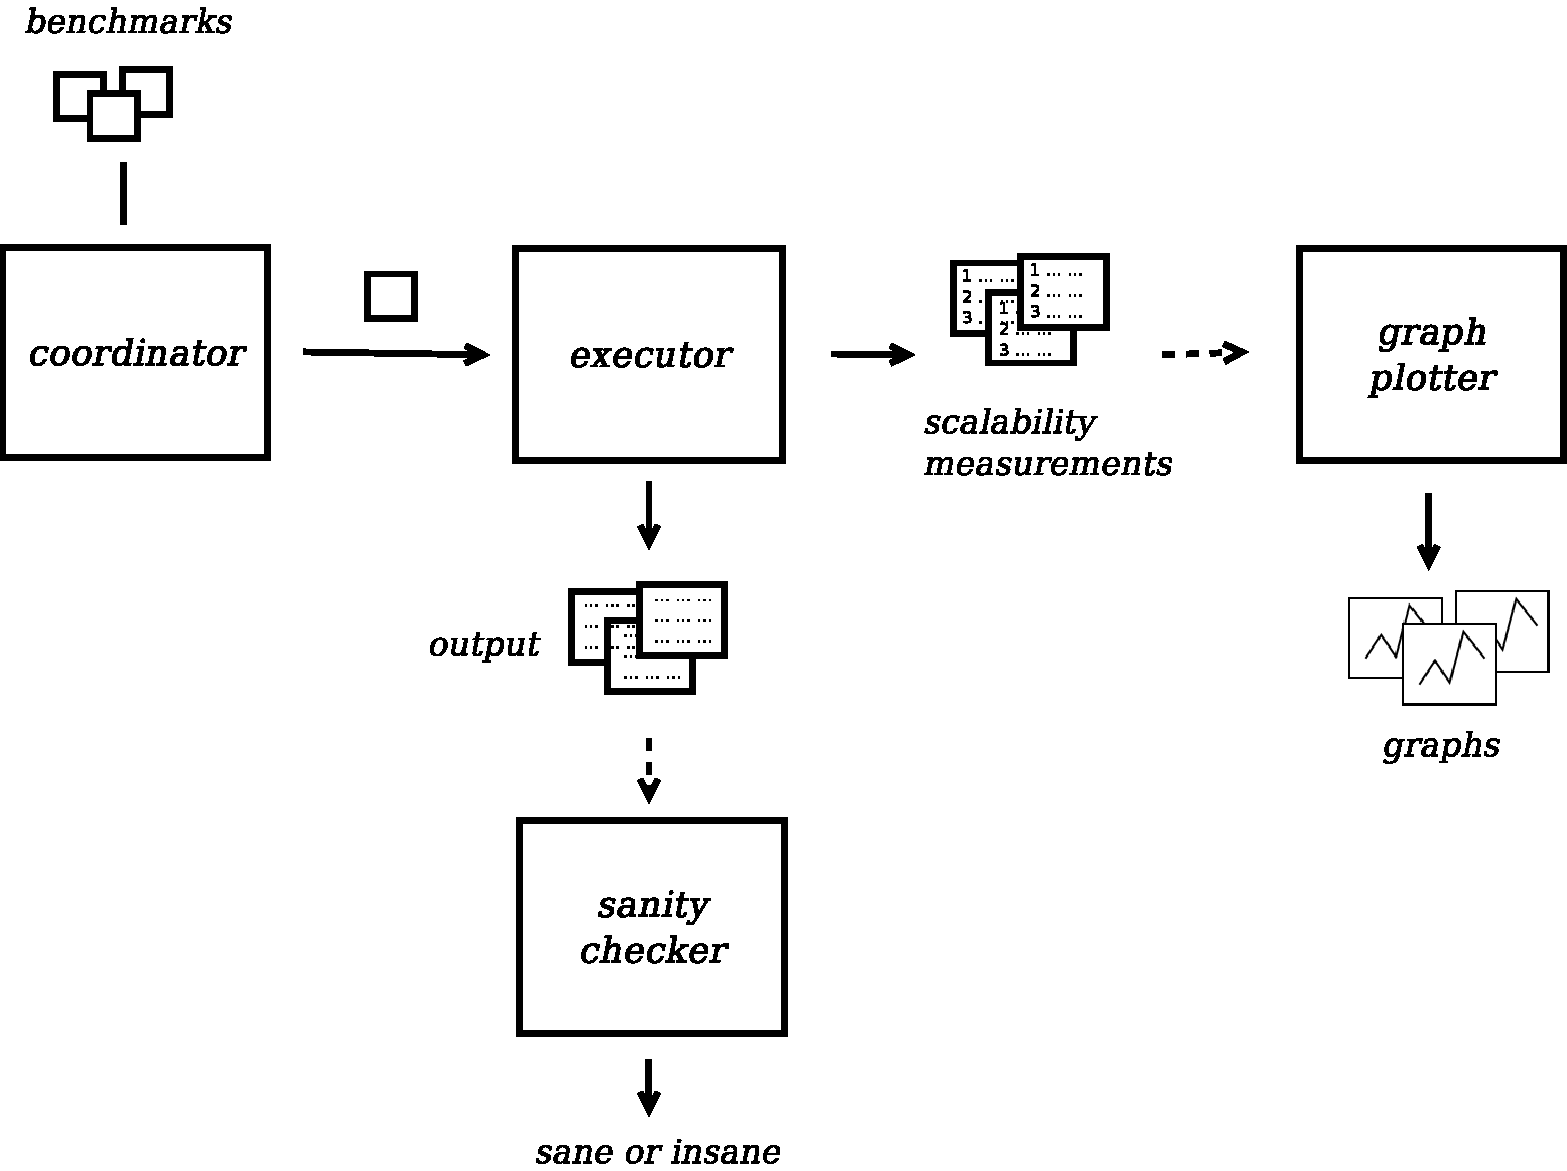
\includegraphics[width=0.8\linewidth]{figures/architecture.pdf}
	\end{center}
\end{frame}

\begin{frame}[fragile]{What does the coordinator do?}
	\begin{verbatim}
   Read global configuration file
   For each benchmark 
      Read benchmark-specific configuration file
      For each runtime environment
         Set up the environment
         Perform any benchmark-specific pre-execution actions
         Prepare a file with instructions for the executor
         Invoke the executor
         Perform any benchmark-specific post-execution actions
      Invoke the sanity checker
      Invoke graph plotter  
	\end{verbatim}
\end{frame}

\begin{frame}{What does the executor do?}
	\begin{verbatim}
   Get the file that the coordinator has prepared
   Start any necessary Erlang slave nodes
   Run the appropriate version of the benchmark
   Stop the Erlang slave nodes
	\end{verbatim}
\end{frame}

\begin{frame}{What does the sanity checker do?}
	\begin{verbatim}
   For each file in the output directory
      Compare it with the rest
      If it differs then
         Insane
   Sane
	\end{verbatim}
\end{frame}

\begin{frame}{What does the graph plotter do?}
	\begin{verbatim}
	\end{verbatim}
\end{frame}

\begin{frame}
\end{frame}

\begin{frame}
\end{frame}

\begin{frame}
\end{frame}

\begin{frame}
\end{frame}

\begin{frame}
\end{frame}

\begin{frame}
\end{frame}

\begin{frame}
\end{frame}

\begin{frame}{Some benchmarks already scale well}
\end{frame}

\begin{frame}{Some benchmarks scale well only in one node}
\end{frame}

\begin{frame}{Some benchmarks do not scale}
\end{frame}

\begin{frame}{Future work}
\end{frame}

\begin{frame}
	\vspace{50pt}
	\begin{center}
	Thank you!
	\end{center}
\end{frame}


\end{document}

